%
\documentclass{bioinfo}
\usepackage{subfigure}
%\usepackage{float}
\usepackage{stfloats}
\usepackage{amsmath}
\usepackage{multirow}
\usepackage[ruled,vlined]{algorithm2e}

\copyrightyear{2012}
\pubyear{2012}

\begin{document}

\firstpage{1}

\title[Optimal Interval Intersection Counting]{
Binary Interval Search (BITS):  \\
A Scalable Algorithm for Counting Interval Intersections}

\author[Layer \textit{et~al}]
{Ryan M. Layer$^1$, 
Kevin Skadron\,$^1$,
Gabriel Robins$^1$, 
and
Aaron Quinlan$^2$\footnote{to whom correspondence should be addressed}}

\address{$^{1}$Department of Computer Science, University of Virginia,
Charlottesville, VA\\
$^{2}$Department of Public Health Sciences and Center for Public Health
Genomics, University of Virginia, Charlottesville, VA}

\history{Received on XXXXX; revised on XXXXX; accepted on XXXXX}

\editor{Associate Editor: XXXXXXX}

\maketitle

\begin{abstract}
\section{Motivation:}
The integration and comparison of diverse genomic datasets is fundamental to
understanding the biology of the genome and the genetic basis of human disease.
Researchers must explore many large datasets of genome intervals (e.g., genes,
polymorphisms, and sequence alignments) in order to place their experiments in a
broader context and make new discoveries.  Relationships between experimental
datasets and genome annotations are typically measured by identifying intervals
that intersect: that is, they overlap and thus share a common genome interval.
Given the continued advances in DNA sequencing technologies, efficient methods
for measuring statistically significant relationships between many, often large,
sets of genomic features is crucial for future discoveries.

\section{Results:}
Here we introduce the Binary Interval Search (BITS) algorithm, a novel and
scalable approach to the interval set intersection problem. Our analyses
demonstrate that BITS excels at counting interval intersections and outperforms
existing methods for the large datasets of common genomic applications.
Moreover, we demonstrate that our algorithm is intrinsically scalable and
well-suited to parallel computing architectures such as Graphics Processing
Units (GPUs). We illustratethe utility of this new algorithm for efficient
Monte-Carlo simulations measuring significant relationships between sets of
genomic intervals.

\section{Availability:}
\href{http://bedtools.googlecode.com}{http://bedtools.googlecode.com}

\section{Contact:} arq5x@virginia.edu
\end{abstract}

\section{Introduction}

Searching for intersecting intervals in multiple sets of genomic features is
crucial to nearly all genomic analyses. For example, interval intersection is
used to compare ChIP enrichment between experiments and cell types, identify
potential regulatory targets, and compare genetic variation among many
individuals.  Interval intersection is the fundamental operation in a broader
class of ``genome arithmetic'' techniques, and, as such, intersection underlies
the functionality found in genome browsers~\citep{kent2002,robinson2011} and
popular analysis software such as SAMTOOLS~\citep{li2009},
BEDTOOLS~\citep{quinlan2010}, GATK~\citep{mckenna2010}, and
GALAXY~\citep{giardine2005}.

As high throughput sequencing technologies have quickly become the 
\emph{de facto} molecular tool for genome biology, the need for efficient
approaches to interval intersection has become increasingly acute. Traditional
techniques for measuring gene expression (e.g., microarrays) and chromatin
states (e.g., ChIP-chip) are being supplanted by sequencing-based techniques
(RNA-seq and ChIP-seq, respectively), and whole-exome and whole-genome
experiments are now routine. Consequently, most genomics labs now conduct
analyses including datasets with millions, if not billions of genome intervals.
Experiments of this size require substantial computation time per pair-wise
comparison, and a typical analysis requires comparisons to many large sets of
genomic features. Existing toolsets for interval intersection scale poorly and
are already reaching their theoretical performance limits. We therefore argue
the need for scalable new algorithms to allow discovery to keep pace with the
scale and complexity of modern datasets.

In this manuscript, we introduce the Binary Interval Search (BITS) algorithm as
a novel and scalable solution to the fundamental problem of counting the number
of intersections between two sets of genomic intervals.  Our algorithm executes
in $\Theta(N \log N)$ time, which can be shown to be optimal for the interval
intersection counting problem by a straight-forward reduction to element
uniqueness (which is known to be $\Theta(N\log N)$~\citep{misra1982}).  We
illustrate that, in the  sequential case, BITS performs similarly to
implementations of traditional algorithms, yet has clear benefits for larger
datasets and for common (e.g., exome sequencing, RNAseq, and ChIPseq) genomic
applications.  Most importantly, we show that the simplicity of the BITS
algorithm is well suited for parallel execution.  The parallel version performs
the same amount of as the single sequential version (i.e., there is no overhead)
which means the algorithm is work-efficient, and because each parallel thread
performs roughly the same amount of work, the algorithm has little thread
divergence. As such the BITS algorithm is a particularly promising approach for
applications requiring large numbers of intersection operations, such as massive
database searches and Monte Carlo measurements of significant relationships
between sets of genome features.

        %%%%%%%%%%%%%%%%%%%%%%%%%%%%%%%%%%%%%%%%%%%%%
        % INTRO: The Interval Set Intersection problem
        %%%%%%%%%%%%%%%%%%%%%%%%%%%%%%%%%%%%%%%%%%%%%
\subsection{The Interval Set Intersection problem}
Before we describe our new approach to interval intersection, we begin by
reviewing some basic definitions.  A genomic \emph{interval} is a single
continuous stretch of a genome with a chromosomal start and end location (e.g.,
a gene), and a genomic \emph{interval set} is a collection of genomic intervals
(e.g., all known genes).  More generally, an interval is the set of all numbers
between a start value and an end value, that can be represented as the pair
$(a.start, a.end)$.  Two intervals $a$ and $b$ {\em intersect} when 
$(a.start \leq b.end)$ and $(a.end \geq b.start)$.  The intersection of two
interval sets $A=\{a_1, a_2, \dots, a_N\}$ and $B=\{b_1, b_2, \dots, b_M\}$ is
the set of interval pairs:

\begin{equation*}
	\begin{split}
		\mathcal{I}(A,B)= &\{ <a,b> | a \in A, b \in B, \\
		& a.start \leq b.end \wedge a.end \geq b.start\}
	\end{split}
\end{equation*}

Intervals within a set can intersect, but {\em self-intersections} are not
included in $\mathcal{I}(A,B)$.  The interval set intersection problem is a
special case of the segment intersection problem where all points are located on
the same line, and each segment belongs to one of two sets. Trere are four
natural sub-problems for interval set intersection.
\begin{enumerate}
	\item The {\em decision problem}
	$\mathcal{I_D}(A,B)$:  given interval sets $A$ an $B$, does there exist at
	least one interval in $A$ that intersects an interval in $B$?

	\item The {\em counting problem}
	$\mathcal{I_C}(A,B)$: how many pair-wise intersections exist between the
	intervals $A$ and $B$? 

	\item The {\em per-interval counting problem}
	$\mathcal{I_P}(A,B)$: how many intervals in $B$ intersect each
	interval in $A$?

	\item The {\em enumeration problem}
	$\mathcal{I}(A,B)$: what is the set of pair-wise interval intersections
	between $A$ an $B$?
\end{enumerate}

While the algorithm we have devised solves all four sub-problems, it is designed
to efficiently \emph{count} the number of intersections between two sets, and as
such, it excels at the \emph{decision}, \emph{counting}, and
\emph{per-interval counting} problems.


%%%%%%%%%%%%%%%%%%%%%%%%%%%%%%%%%%%%%%%%%%%%%%%%%%%%%%%%%%%
% INTRO: Parallelization limitations of existing approaches
%%%%%%%%%%%%%%%%%%%%%%%%%%%%%%%%%%%%%%%%%%%%%%%%%%%%%%%%%%%
\subsection{Limits to parallelization}

Interval intersection has many applications in genomics, and as such, several
algorithms have been developed that, in general, are either based on
trees~\citep{kent2002}, NCLists~\citep{alekseyenko2007}, or linear sweeps of
pre-sorted intervals~\citep{richardson2006}.

The UCSC genome browser introduced a clever and now widely-used scheme based on
R-trees. This binning approach partitions intervals from one dataset into
hierarchical ``bins''.  Intervals from a second dataset are then compared solely
to matching bins (instead of the entire dataset) in order to narrow the search
for intersections to a focused portion of the genome.  While this popular
approach is used by the Kent tools software, BEDTools~\citep{quinlan2010},
SAMTOOLS~\citep{li2009}, and TABIX~\citep{li2011}, the algorithm is inefficient
for counting intersections since all intervals in each candidate bin must be
enumerated to count the intersections.

Moreover, these existing approaches are poor candidates for parallelization.
Thread divergence can be a significant problem for hierarchical binning methods
such as the UCSC binning algorithm.  If intervals are not uniformly distributed
(e.g., exome sequencing or RNA-seq), then a small number of bins will contain
many intervals while other bins are empty. Consequently, threads searching full
bins will take substantially longer than threads searching empty bins.  In
contrast, BITS can count intersections directly without the need to enumerate
intersecting intervals and therefore, the underlying interval distribution does
not impact the relative workload of each thread.

% Binning the hierarchical binning data structure can also be difficult to build
% in some parallel architectures.  For example, in NVIDIA's CUDA at least one
% extra passes over the interval database is required to allocate the correct
% amount of space for each bin.  BITS uses integer arrays, which easily map to
% most architectures.

Recent versions of BEDTools and BEDOPS~\citep{neph2012} conduct a
linear ``sweep'' through pre-sorted datasets while maintaining an auxiliary
data structure to track intersections as they are encountered. While the
complexity of such sequential sweep algorithms is theoretically optimal, the 
amount of parallelism that exists is limited, and some overhead is required to
guarantee correctness.  Any linear sweep algorithm must maintain the ``sweep
invariant''~\citep{mckenney2009}, which states that all segment starts, ends, 
and intersections behind the sweep must be known.  A parallel sweep algorithm
must either partition the input space such that each section can be swept in
parallel without violating the invariant, or threads must communicate 
about intervals that span partitions.  In the first case parallelism is limited
to the number of partitions that can be created, and threads can diverge when 
the number of intervals in each partition are unbalanced.  In the second case,
the communication overhead between threads prevents work efficiency and can 
have significant performance implications.

% Several parallel sweep algorithms have been proposed~\citep{goodrich1993,
% kriegel1991, mckenney2009} for segment intersection (a generalization of
% interval intersection), but they all depend on a partitioned input space
% scheme and thus have limited parallelism and increased overhead.


%%%%%%%%%%%%%%%%%%%%%%%%%%%%%%%%%%%%%%%%%%%%%%%%%%%%%%%%
% METHODS
%%%%%%%%%%%%%%%%%%%%%%%%%%%%%%%%%%%%%%%%%%%%%%%%%%%%%%%%
\section{Methods}

%%%%%%%%%%%%%%%%%%%%%%%%%%%%%%%%%%%%%%%%%%%%%%%%%%%%%%%%
% METHODS: BITS
%%%%%%%%%%%%%%%%%%%%%%%%%%%%%%%%%%%%%%%%%%%%%%%%%%%%%%%%

A seemingly facile method for finding the intersection of $A$ and $B$ would be
to treat one set, $A$, as a "query" set, and the other, $B$, as a "database". If
all of the intervals in the database were sorted by their starting coordinates,
it would seem that binary searches could be used for each query interval to
identify all of the intersecting database intervals. Formally, such a
"searching" algorithm would return, for each interval $a_i \in A$, the set of
intervals in $B$ that intersect $a_i$.

However, this apparently straight-forward searching algorithm is complicated by
a subtle, yet vexing detail. If the intervals in $B$ are sorted by their
starting positions, then a binary search of $B$ for the query interval end
position $a_i.end$ will return the interval $b_j \in B$, where $b_j$ is the last
interval in $B$ that starts before interval $a_i$ ends (e.g, interval $e$ in
Fig. 1A).  This would seem to imply that if $b_j$ does not intersect $a_i$, then
no intervals in $B$ intersect $a_i$, and if $b_j$ does intersect $a_i$, then
other intersecting intervals in $B$ could be found by scanning the intervals
starting before $b_j$ in decreasing order, stopping at the first interval that
does not intersect $a_i$.  However, this technique is complicated by the
possibility of intervals that are wholly {\em contained} inside other intervals
(e.g., interval \emph{c} in Fig. 1B). 

An interval $b_j\in B$ is ``contained'' if there exists an interval $b_k \in B$
where $b_k.start \leq b_j.start$ and $b_j.end \leq b_k.end$.  Considering such
intervals, if the interval found in the previous binary search $b_j$ does not
intersect the query interval $a_i$, we cannot conclude that no interval in $B$
intersects $a_i$, because there may exist an interval $b_{j-x} \in B$ where
$b_{j-x}.end > a_i.start$.  Furthermore, if $b_j$ does intersect $a_i$, then the
subsequent scan for other intersecting intervals cannot stop at the first
interval that does not intersect $a_i$; it is possible that some earlier
containing interval intersects $a_i$. Therefore, the scan is forced to continue
until it reaches the beginning of the list. As wholly-contained intervals are
commonplace for genomic datasets, a naive binary search solution is inviable.

\begin{figure}[h]
		\centering
		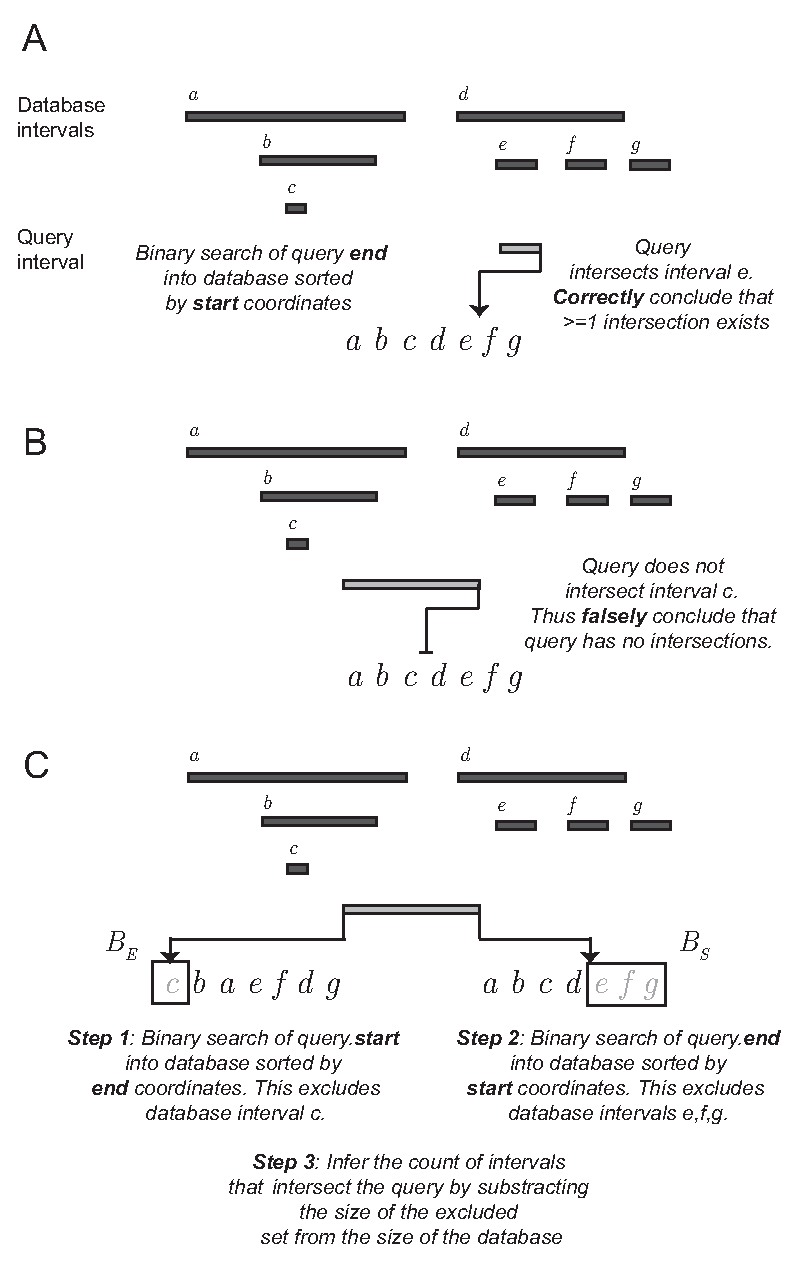
\includegraphics[width=3in]{figures/Figure1.v3.eps}
		\caption{TO DO.}
		\label{bitssearching}
\end{figure}

        
\subsection{Binary Interval Search (BITS) Algorithm}
We now introduce our new Binary Interval Search (BITS) algorithm for solving the
interval set intersection problem.  This algorithm uses binary searches to
identify interval intersections while avoiding the aforementioned complexities
caused by contained intervals. The key observation underlying the BITS algorithm
is that the \emph{size} of the intersection between two sets can be determined
without enumerating each intersection.  For each interval in the query set, two
binary searches are performed to determine the number of intervals in the
database that intersect the query interval.  Each pair of searches is
independent of all others, and thus all searches can be performed in parallel.  

Previously, the intersecting set was defined based on \emph{inclusion}: that is,
the set of intervals in the interval database $B$ that end after the query
interval $a_i$ begins, and which begin before $a_i$ ends.  However, contained
intervals make it difficult to find this set directly.  The search for the
intersecting intervals can start at the interval in $B$ closest to $a_i$, but
must continue to the beginning of $B$ because there is no condition indicating
that all intersecting intervals have been found.  By restating the intersection
definition, we are able to determine the size of the intersecting set, which
provides a terminating condition for the search, so that it may stop once the
last interval in the intersecting set has been found.

Our algorithm uses a different, but equivalent, definition of interval
intersection based on \emph{exclusion}: that is, by identifying the set of
intervals in $B$ that \emph{cannot} intersect $a_i$, we can infer how many
intervals \emph{must} intersect $a_i$. Formally, we define the set of intervals
$\mathcal{I}(B,a_i) \in B$ that intersect query interval $a_i\in A$ to be the
intervals in $B$ that are neither in the set of intervals ending before ("left
of", set $L$ below) $a_i$ begins, nor in the set of intervals starting after
("right of", set $R$ below) $a_i$ ends.  That is:
\begin{equation*}
	\begin{split}
		\mathcal{L}(B,a_i) = &\{b\in B| b.end < a_i.start\} \\
		\mathcal{R}(B,a_i) = &\{b\in B| b.start > a_i.end\} \\
		\mathcal{I}(B,a_i) = &B / (\mathcal{L}(B,a_i) \cup \mathcal{R}(B,a_i))
	\end{split}
\end{equation*}

Finding the intervals in $\mathcal{I}(a_i,B)$ for each $a_i\in A$ by taking the
difference of $B$ and the union of $\mathcal{L}(B,a_i)$ and $\mathcal{G}(B,a_i)$
is not efficient.  However, we can quickly find the size of $\mathcal{L}(B,a_i)$
and the size $\mathcal{G}(B,a_i)$, then \emph{infer} the size of
$\mathcal{I}(B,a_i)$.  With the size of $\mathcal{I}(B,a_i)$, we can directly
answer the decision problem, the counting problem, and the per-interval counting
problems.
% Moreover, the size can also serve as the previously missing (see section 1.1)
% terminating condition in the enumeration problem.

\begin{algorithm}[h]
	\DontPrintSemicolon
	\footnotesize
	\KwIn{Sorted interval starts and ends $B_S$ and $B_E$, query interval $a$}
	\KwOut{Number of intervals $c$ intersecting $a$}
	\BlankLine
	\textbf{Function} \textsc{ICount}$(B_S,B_E,a)$
	\Begin {
		$first \gets \textsc{BSearch}(B_S, a.end)$\;
		$last \gets \textsc{BSearch}(B_E, a.start)$\;
		$c \gets first - last$\;
		\Return $c$\;
	}
	\caption{Single interval intersection counter}
\end{algorithm}

The core function in our algorithm 
$\textsc{ICount}(B_S,B_E,a_i) = |\mathcal{I}(B,a_i)|$ determines the number of
intervals in the database $B$ that intersect query interval $a_i$.  As shown in
Fig. 1C, the database $B$ is split into two integer lists
$B_S = [b_1.start, b_2.start, \dots, b_M.start]$ and 
$B_E = [b_1.end, b_2.end, \dots, b_M.end]$, which are each are sorted
numerically in ascending order.  Next, two binary searches are performed,
$last=\textsc{ BSearch}(B_E, a_i.start)$ and 
$first=\textsc{ BSearch}(B_S, a_i.end)$.  Since $B_E$ is a sorted list of each
interval end coordinate in $B$, the elements less than or equal to $last$ in
$B_E$ correspond to the set of intervals in $B$ that end \emph{before} $a_i$
starts (i.e., to the "left" of).  Similarly, the elements greater than or equal
to $first$ in $B_S$ correspond to the set of intervals in $B$ that start
\emph{after} $a_i$ ends (i.e., to the "right" of).  From these two values, we
can directly infer the size of the intersection set $\mathcal{I}(B,a_i)$ (i.e.,
the \emph{count} of intersections in $B$ for $a_i$z):
\begin{equation*}
	\begin{split}
		|B|-first=&|\mathcal{R}(B,a_i)| \\
		last=&|\mathcal{L}(B,a_i)| \\ 
		|B|-(last+(|B|-first))=&|\mathcal{I}(B,a_i)|
	\end{split}
\end{equation*}

% As mentioned, this problem cannot be solved with a single sorted list because
% contained intervals prevent the total ordering of $B$. If $B$ is sorted by
% interval start coordinates, then the interval end coordinates may be unordered
% and $last$ cannot be found efficiently.  Similarly, if $B$ is sorted by
% interval end, $first$ can not be found efficiently.

Using the subroutine $\textsc{ICount}(B_S,B_E,a_i)$ as the core operation in
BITS, all four interval set intersection problem variants can be solved
(pseudocode for the \emph{decision} and \emph{enumeration} sub-problems can be
found in the Supplemental Materials):

\begin{enumerate}

	% \item
	% {\em Decision problem:} Let $c$ be an accumulator variable that is
	% initialized to zero; then for each $a_i \in A$, accumulate $c = c +
	% \textsc{ICount}(B_S,B_E,a_i)$.  If $c\ne0$ return {\em yes}, otherwise
	% return {\em no}.

	\item {\em Counting problem:}
	Let $c$ be an accumulator variable that is initialized to zero; then for
	each $a_i \in A$, accumulate $c = c + \textsc{ICount}(B_S,B_E,a_i)$.  The
	total accumulated count $c$ is returned.
	\begin{algorithm}[h]
		\DontPrintSemicolon
		\footnotesize
		\KwIn{Database intervals array $B$ and query interval array $A$}
		\KwOut{Number of intersections $c$ between $A$ and $B$}
		\BlankLine
		\textbf{Function} \textsc{Counter}$(A,B)$
		\Begin {
			$B_S \gets [b_1.start, \dots, b_M.start]$ where $|B| = M$\;
			$B_E \gets [b_1.end, \dots, b_M.start]$ where $|B| = M$\;
			\textsc{Sort}($B_S$)\;
			\textsc{Sort}($B_E$)\;
			$c \gets 0$\;
			\For{$i \gets 1$ \KwTo $|A|$} {
				$c \gets c + \textsc{ICount}(B_S,B_E,A[i])$
			}
			\Return $c$\;
		}
		\caption{Interval intersection counter}
	\end{algorithm}
	
	\item {\em Per-interval counting problem:}
	Let $C$ be an accumulator array where element $C[i]$ corresponds to the
	number of intersection for each element in $a_i\in A$.  For each 
	$a_i \in A$, set $C[i]=\textsc{ICount}(B_S,B_E,a_i)$.  The total list of
	counts $C$ is then returned.
	\begin{algorithm}[h]
		\DontPrintSemicolon
		\footnotesize
		\KwIn{Database intervals array $B$ and query intervals array $A$}
		\KwOut{Array of intersections counts $C$ where $|C|=|A|$}
		\BlankLine
		\textbf{Function} \textsc{PerIntervalCounter}$(A,B)$
		\Begin {
			$B_S \gets [b_1.start, \dots, b_M.start]$ where $|B| = M$\;
			$B_E \gets [b_1.end, \dots, b_M.start]$ where $|B| = M$\;
			\textsc{Sort}($B_S$)\;
			\textsc{Sort}($B_E$)\;
			$C \gets [0, \dots, 0]$\;
			\For{$i \gets 1$ \KwTo $|A|$} {
				$C[i] \gets \textsc{ICount}(B_S,B_E,A[i])$
			}
			\Return $C$\;
		}
		\caption{Per interval intersection counter}
	\end{algorithm}

	% \item
	% {\em Enumeration problem:} First find the per-interval counting array
	% $C=\textsc{PerIntervalCounter}(A,B)$ then the let $R$ be the prefix sum
	% (\textbf{WHAT DOES PREFIX SUM MEAN?)}) of $C$. The array $R$ is used to
	% track the number of intervals that must be found in each of the subsequent
	% scans.  Let $start = 0$ track the number of enumerated intersections.  For
	% $i=1\dots|A|$, let $end = R[i]$ where $end - start$ is the number
	% intervals in $B$ that intersect $a_i$.  Let $from=\textsc{BSearch}(B_S,
	% a_i.end)$ be the initial position of the scan.  While $end - start > 0$
	% some number of intervals in $B$ must be scanned for an intersection with
	% $a_i$.  If $a_i$ intersections $b_from$ then let $E[start] = <a_i,
	% b_from>$ and $start=start+1$.  Then let $from = from +1$.  Finally, the
	% total set of intersecting intervals $E$ is returned (\textbf{Algorithm
	% 4}).
\end{enumerate}
        

        % \begin{algorithm}[h]
        %       \DontPrintSemicolon
        %       \footnotesize
		%       \KwIn{Database intervals array $B$ and query intervals array
		%       $A$} \KwOut{Array of pair-wise intersections $E$ }
        %       \BlankLine
        %       \textbf{Function} \textsc{Enumerator}$(A,B)$
        %       \Begin {
        %       $B_S \gets [b_1.start, \dots, b_M.start]$ where $|B| = M$\;
        %       $B_E \gets [b_1.end, \dots, b_M.start]$ where $|B| = M$\;
        %       \textsc{Sort}($B_S$)\;
        %       \textsc{Sort}($B_E$)\;
        %       $C \gets \textsc{PerIntervalCounter}(A,B)$\;
        %       $R \gets \textsc{PrefixSum}(C)$\;
        %       $E \gets [<0,0>, \dots, <0,0>]$\;
        %       $start \gets 0$\;
        %       \For{$i \gets 1$ \KwTo $|A|$} {
        %       $end \gets R[i]$\;
        %       $from \gets \textsc{BSearch}(B_S, A[i].end)$\;
        %       \While{$end - start > 0$}{
        %       \If{ $A[i]$ intersects $B[from]$}{
        %       $E[start] = <A[i], B[from]>$\;
        %       $start \gets start + 1$\;
        %       }               
        %       $from \gets from - 1$\;
        %       }
        %       }
        %       \Return $E$\;
        %       }
        %       \caption{Intersection enumerator}
        % \end{algorithm}

%%%%%%%%%%%%%%%%%%%%%%%%%%%%%%%%%%%%%%%%%%%%%%%%%%%%%%%%
% METHODS: TIME COMPLEXITY ANALYSIS
%%%%%%%%%%%%%%%%%%%%%%%%%%%%%%%%%%%%%%%%%%%%%%%%%%%%%%%%
\subsection{Time Complexity Analysis}

To compute $\textsc{ICount}(B_S,B_E,a_i)$ for each $a_i$ in $A$, the interval
set $B$ is first split into two sorted integer lists $B_S$ and $B_E$, which
requires $O(|B| \log |B|)$ time.  Next, each instance of
$\textsc{ICount}(B_S,B_E,a_i)$ searches both $B_S$ and $B_E$, which consumes
$O(|A| \log |B|)$ time.  For the counting problems, combining the results of all
$\textsc{ICount}(B_S,B_E,a_i)$ instances into a final result can be accomplished
in $O(N)$ time.  

% The total complexity of the counting problems is therefore $O((|A| + |B|) \log
% |B|)$.  The enumeration problem requires additional steps to scan the
% intervals in $B_S$.  In the best case scenario, each scan requires
% $\textsc{ICount}(B_S,B_E,a_i)$ extra steps, to a total of $O(|B| \log |B| +
% C)$ time, where is $C$ is the number of intersections.  However, contained
% intervals can cause the scan to process more than $C$ elements.  If there
% exists some $a_i$ that intersects $b_{j}$ and $b_{j-2}$, but not $b_{j-1}$
% (i.e., $b_{j-2}$ contains $b_{j-1}$), then the enumeration scan will consider
% one extra element, namely $b_{j-1}$.  In the pathological case, $b_0$ contains
% intervals $\{b_1, \dots, b_N\} \in B$, $a_i$ intersects $b_0$, and $a_i$
% starts after interval $b_N$ ends.  This scenario would cause the enumeration
% scan to consider all the elements in $B$.  If all $a_i$ in $A$ are
% pathological, then each scan would required $|B|$ extra steps, to a total of
% $O(|B| \log |B| + |A||B|)$ time.


%%%%%%%%%%%%%%%%%%%%%%%%%%%%%%%%%%%%%%%%%%%%%%%%%%%%%%%%
% METHODS: Parallel BITS
%%%%%%%%%%%%%%%%%%%%%%%%%%%%%%%%%%%%%%%%%%%%%%%%%%%%%%%%
\subsection{Parallel BITS}

Performing a single operation independently on many different inputs is a
classic parallelization scenario.  When based on the subroutine
$\textsc{ICount}(B_S,B_E,a)$, which is independent of all
$\textsc{ICount}(B_S,B_E,b)$ for intervals $b$ in the query set where $a \neq
b$, counting interval intersections is a {\em pleasingly parallelizable} problem
that easily maps to a number of parallel architectures.

NVIDIA's Compute Unified Device Architecture (CUDA) is a single instruction
multiple data (SIMD) architecture that provides programmers a general interface
to a large number of parallel graphics processing units (GPUs).  The BITS
algorithm is especially well suited for the NVIDIA CUDA architecture for a
number of reasons.  First, CUDA is optimized to handle large numbers of threads.
By assigning each thread one instance of $\textsc{ICount}(B_S,B_E,a)$, the
number of threads will be proportional to the file size.  CUDA threads also
execute in lock-step and any divergence between threads will cause reduced
thread utilization.  While there is some divergence in the depth of each binary
search performed by $\textsc{ICount}(B_S,B_E,a)$, it has an upper bound of
$O(log |B|)$.  Outside of this divergence $\textsc{ICount}(B_S,B_E,a)$ is a
classic SIMD operation~\citep{kirk2010}.  Finally, the only data structure
required for this algorithm is a sorted array.  Sorting on GPU has been an
active area of research for many years, and current GPU sorting algorithms can
sort billions of integers within seconds~\citep{merrill2011}.

%%%%%%%%%%%%%%%%%%%%%%%%%%%%%%%%%%%%%%%%%%%%%%%%%%%%%%%%
% RESULTS
%%%%%%%%%%%%%%%%%%%%%%%%%%%%%%%%%%%%%%%%%%%%%%%%%%%%%%%%
\section{Results}

%%%%%%%%%%%%%%%%%%%%%%%%%%%%%%%%%%%%%%%%%%%%%%%%%%%%%%%%
% RESULTS: Comparing sequential BITS to existing approaches
%%%%%%%%%%%%%%%%%%%%%%%%%%%%%%%%%%%%%%%%%%%%%%%%%%%%%%%%
\subsection{Comparing sequential BITS to existing approaches}
We implemented a sequential version of the BITS algorithm as a standalone C/C++
utility using our BEDTools~\citep{quinlan2010} genome arithmetic suite. Here we
assess the performance of this sequential implementation relative to the
BEDTOOLS \texttt{intersect} and UCSC Genome Browser's ("UCSC") \citep{kent2002}
\texttt{bedIntersect} utilities (\textbf{see Suppl. Methods - describe commands,
how we did timing, what machine, CPU, GPU, startup-time, etc.}).  We compare the
performance of each tool for \emph{counting} the total number of observed
intersections between sets of intervals of varying sizes (Figure 2). The
comparisons presented are based sequence alignment intervals extracted from
datasets created for the CEU individual NA12878 by the 1000 Genomes
Project\textbf{TO: CITE}), as well as RefSeq exons (N=400,531). Owing to the
different data structures used by each algorithm, the relative performance of
each approach may depend on the genomic distribution of intervals within the
sets.  For example, tree-based solutions (i.e., BEDTools and UCSC) placing
intervals into hierarchical bins may perform poorly when intervals are unevenly
distributed among the bins. To test the effect of differing interval
distributions on algorithm performance, we randomly sampled 1 and 10 million
alignment intervals from both whole-genome and exome-capture datasets for this
individual (see Supplemental Methods). Each algorithm was evaluated considering
three different interval intersection scenarios:

\begin{figure*}[btp]
	\centering
	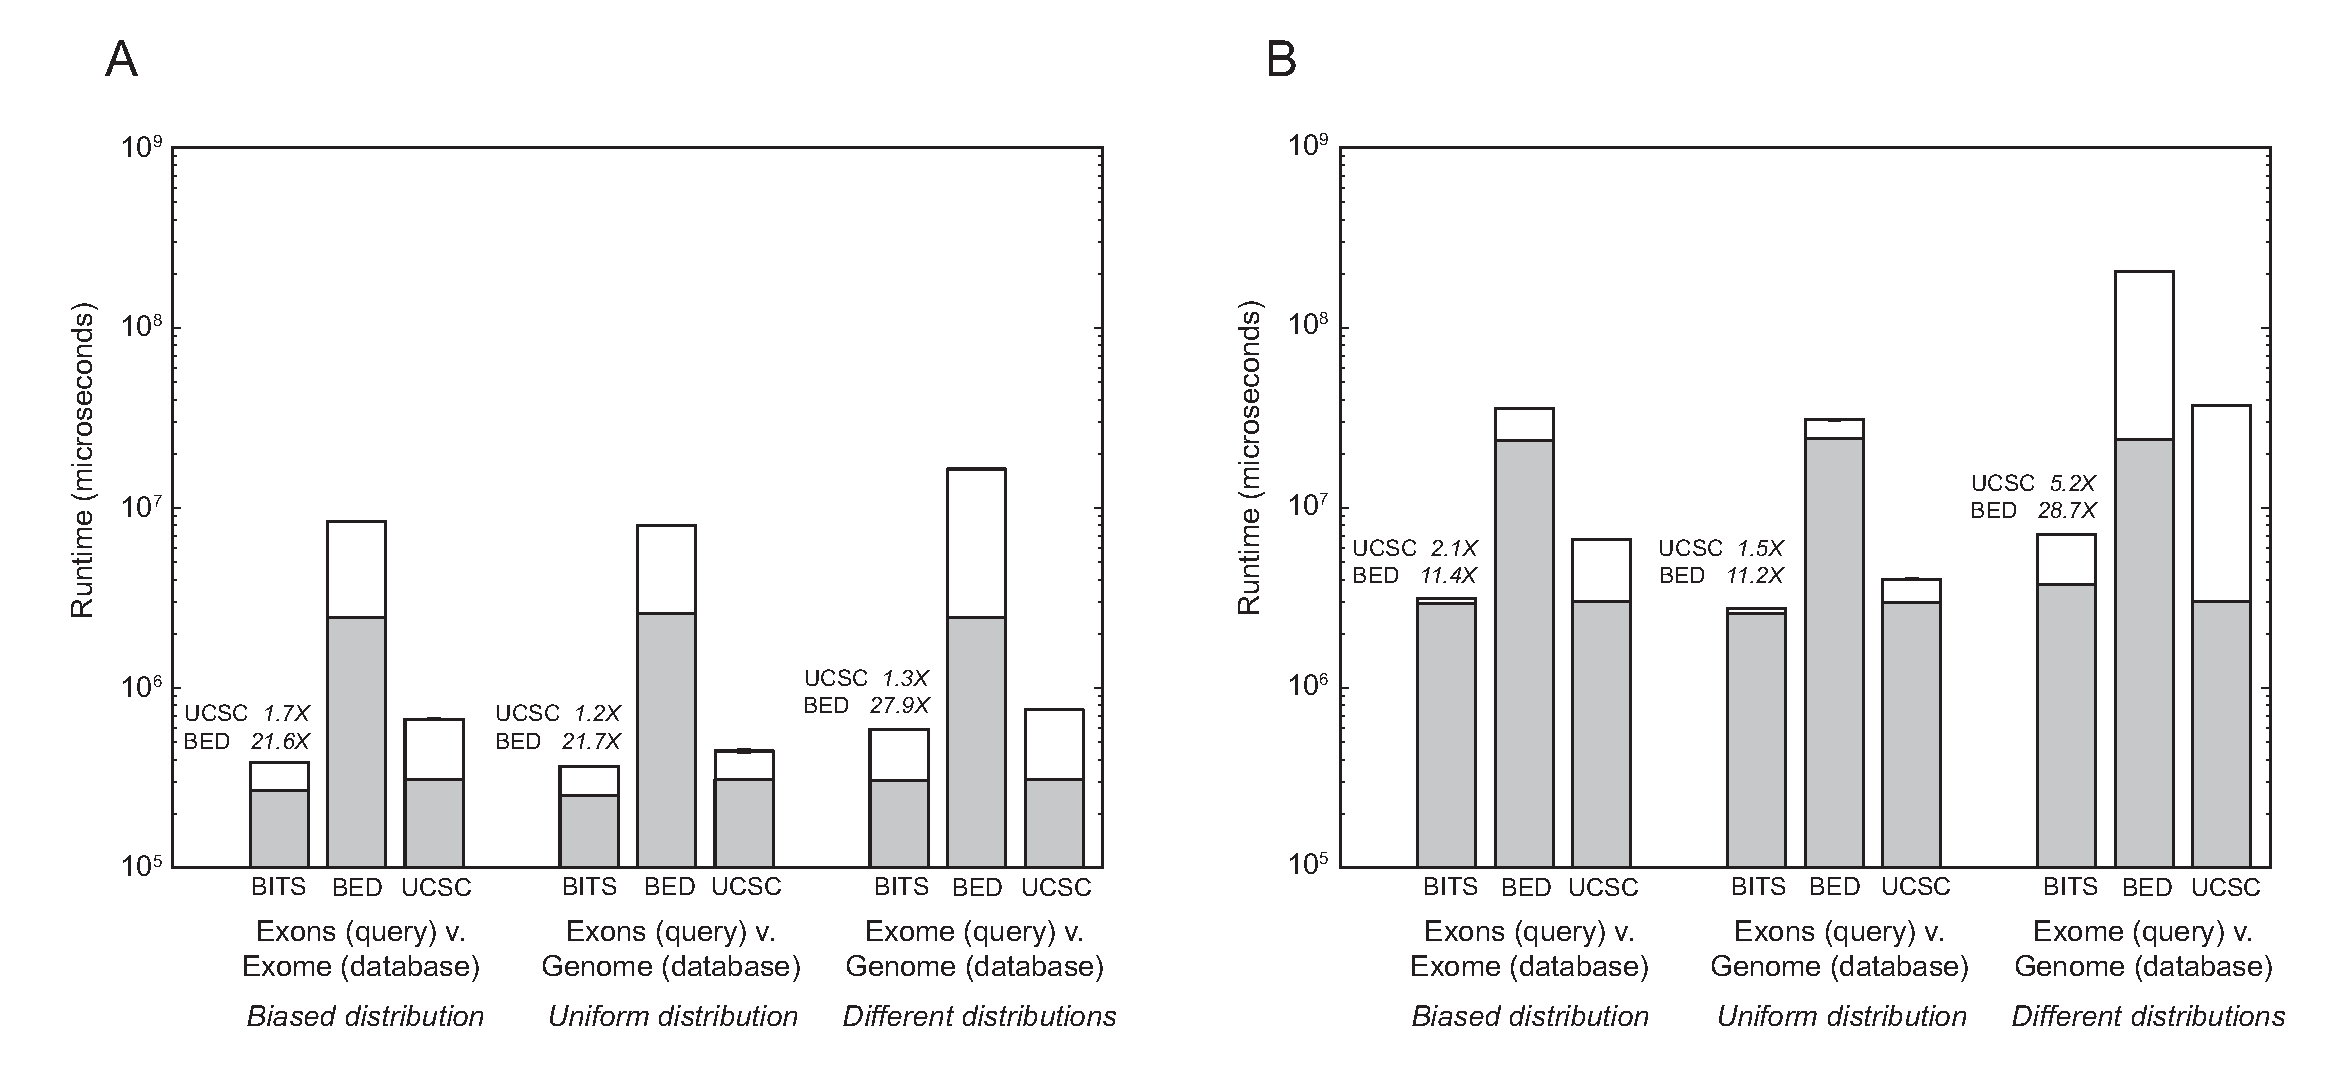
\includegraphics[width=7in]{figures/seq-counting.eps}
	\caption[]{Run times for counting intersections with 
	BITS, BEDTools, and UCSC "Kent source".  \textbf{A}. Run times for databases
	of 1 million alignment intervals from each interval distribution.
	\textbf{B}.  Run times for databases of 10 million alignment intervals from
	each interval distribution.  In each case, the bars reflect the mean run
	time from five independent experiments and error bars describe the standard
	deviation.  Graybars reflect the portion of the run time consumed by
	constructing the data structures required for intersection, while white bars
	indicate the time spent on counting intersections.  Above each BITS
	execution time we note the speed increase relative to BEDTools and "Kent
	source", respectively. "Exons" represents 400,351 RefSeq exons (autosomal
	and X, Y) for the human genome (Build 37).  BED = BEDTools; UCSC = "Kent
	source"}
\end{figure*}

\begin{enumerate}
	\item {\em Intervals from different distributions}:
	the intersection between exome-capture alignments and whole-genome
	alignments. Since the interval sets have a large number of intervals and
	each set has a different genomic distribution, we expect a small number of
	intersections.
	
	\item {\em Uniform interval distribution}:
	the intersection between Refseq exons and genome-wide sequencing data.
	Since each interval set is, for the most part, evenly distributed throughout
	the genome, we expect that each exon will intersect roughly the same number
	of sequencing intervals, and a large number of sequencing intervals will not
	intersect an exon.

	\item {\em Biased interval distribution}:
	the intersection between exons and exome-capture alignments. By design, 
	exome sequencing experiments intentionally bias DNA sequences to the coding
	exons. Thus, the vast majority of sequence intervals will align in exonic
	regions. In contrast to the previous scenario, nearly every exon interval
	will have a large number of sequence interval intersections, and nearly all
	sequencing intervals will intersect an exon.
\end{enumerate}
        
\subsubsection{BITS excels at counting intersections}

In all three interval distribution scenarios, the sequential version of BITS had
superior runtime performance for counting intersections.  BITS was between 11.2
and 27.9 times faster than BEDTools and between 1.2 and 5.2 times faster than
UCSC (Figure 2). This behavior is expected; whereas the BEDTools and UCSC
tree-based algorithms must \emph{enumerate} each intersection in order to derive
the \emph{count} of intersections, BITS can \emph{infer} the intersection count
by exclusion without enumeration.

\subsubsection{BITS outperforms for large intersections and biased data
distributions.}
The relative performance gains of the BITS approach are enhanced for very large
datasets (Figure 2B), as the tree-based methods will, on average, have a large
number of intervals in each queried bin. In contrast, since BITS is based on
binary search ($O(\log |B|)$ complexity), its performance scales more linearly
with respect to dataset size.

Similarly, datasets such as exome-capture experiments lead to biased
distributions of intervals among the UCSC bins. Consequently, most bins in
tree-based methods will contain no intervals, while a small fraction contain
many intervals. When the query intervals have the same bias, the overhead of the
UCSC algorithm is more onerous, as a small number of bins are queried and each
queried bin contains many intersecting intervals that must be enumerated in
order to count overlaps. As the BITS algorithm is agnostic to the interval
distributions, it will outperform the UCSC algorithm (Figure 2A, 2B) for common
genomic analyses such as ChIP-seq, RNA-seq, and CNV detection, especially for
the typically large sequence alignment datasets that these experiments generate.

% \begin{figure}[h]
%   \centering
%   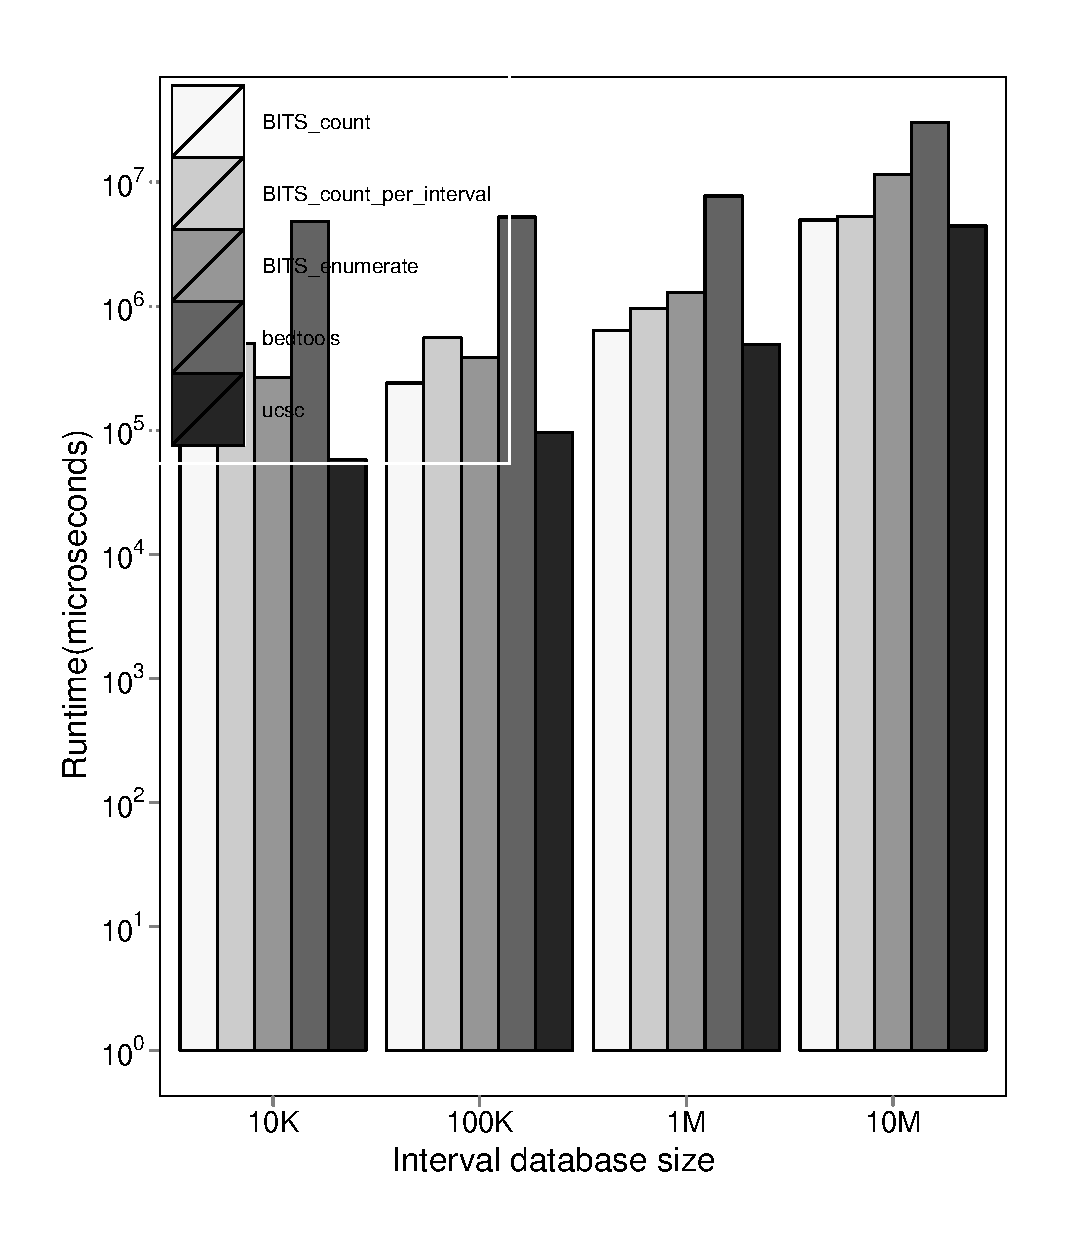
\includegraphics[width=3in]{figures/exons-v-genome.eps}
%   \caption[]{Run times for each algorithm using exons and whole-genome datasets (FIX: caption and need error bars).}
% \end{figure}


% \begin{figure}[h]
%   \centering
%   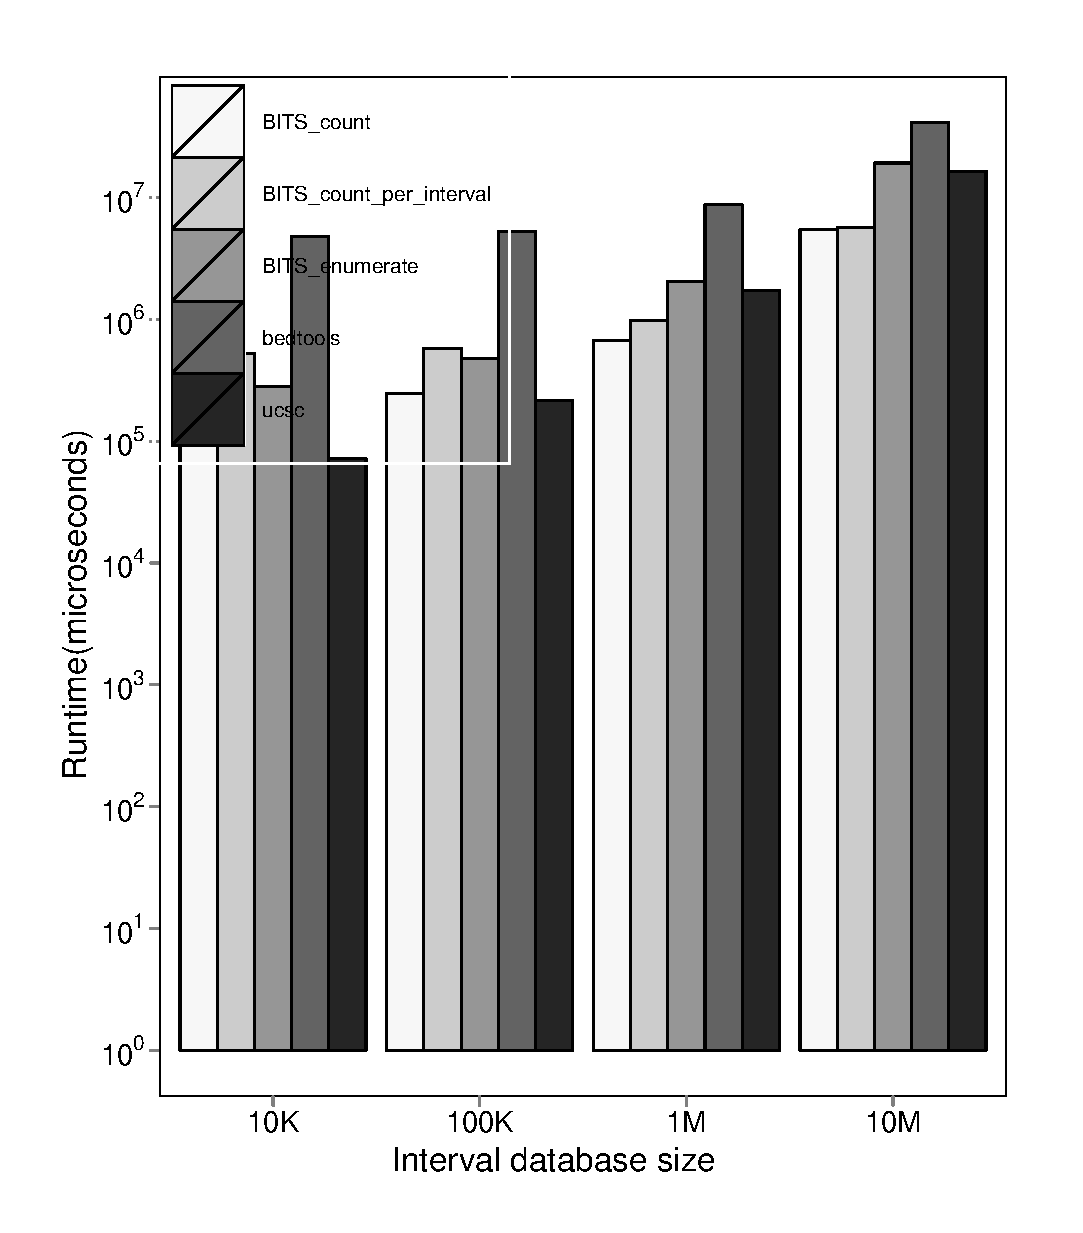
\includegraphics[width=3in]{figures/exons-v-exome.eps}
%   \caption[]{Run times for each algorithm using exons and whole-exome datasets (FIX: caption and need error bars).}
% \end{figure}

% the primary functions used to analyze large data sets.  For
% example, the utility of the full list of 9,148,823 intersection between human
% exon and the exome sequencing of the NA12878 individual (the biased distribution
% scenario) is limited, while the number of intersections per exon can provide
% insight into deletions, duplications, and other properties of NA12878's
% genome.
% 
% The performance profiles of counting (Figure~\ref{count}) and per interval
% counting (Figure~\ref{perintervalcount}) were similar for all algorithms.
% In these two scenarios, excluding the smallest data sets, all versions of BITS
% performed faster than both Kent tools and BEDTools.  For the 10K database, Kent
% tools performed faster than the sequential and OpenMP version of BITS by up to a
% factor of three.  The following table gives the average speedups of the three
% versions of BITS over Kent tools and BEDTools for the 10 million interval
% database.
% 
% For enumeration, the performance improvements of the  sequential and OpenMP
% versions of BITS were an order of magnitude lower against BEDTools, and
% non-existent against Kent tools.  In fact, Kent tools performed better than
% sequential BITS by a factor of nearly three for the smallest database
% (Figure~\ref{fig:eexonfull}), and the run times of the two where nearly
% equivalent for the largest database.  The CUDA version of BITS did provide a
% modest improvement over both Kent tools and BEDTools, but at a level lower than
% in counting and per interval counting.
% The following table  gives the average speedups of the three versions of BITS
% over Kent tools and BEDTools for the 10 million interval database.
% All run-times were measured on a 2.66 GHz quad-core Intel Xeon X555 CPU with 8
% MB of cache running Ubuntu Linux version 4.4.3 (kernel version 2.6.32-34).
% Run-times for CUDA were measured on an NVIDIA Tesla C2050 GPU with 448 1.15 GHz
% cores, 3 GB of global memory, CUDA driver version 4246739, and CUDA runtime
% version 4.0.  The source code was compiled using gcc version 4.4.3, and NVIDIA
% CUDA compilation tools release 4.0, V0.2.1221.  In each case, run-times measure 
% the performance of the intersection algorithm and thus do not include disk
% reading, writing, or the time required to initialize the GPU.

% The results of our tests are given in Figure~\ref{count},
% Figure~\ref{perintervalcount}, and Figure~\ref{enumerate}.


% In nearly every case, the sequential version of BITS outperformed both Kent
% tools and BEDTools.  The most striking improvement was in the interval
% counting operation, where ---in the largest operation (10M many short
% intervals, a total of 2e$^7$ intervals)--- sequential BITS achieved a speedup
% of 7.7x over Kent tools and 27.4x over BEDTools.  In this same case the
% speedup over Kent tools and BEDTools by OpenMP BITS was 13.1x and 46.6x, and
% the speedup by CUDA BITS was 143.7x and 508.8x, respectively.
% 
% While BITS did have some improvement in enumeration operation, the speedup was
% an order of magnitude lower than in the counting operations, and Kent tools
% performed better than sequential bits in one scenario.  This result is
% expected given that BITS is optimized for counting intersections, which is
% generally more a useful operation in large-scale comparisons.

%\begin{table}[h] \caption{Average speedup for intersection counting and per
%interval counting for the 10M database}
%\centering
% \begin{center}
%       \begin{tabular}{lll}
%               \\
%               & Kent tools & BEDTools \\
%               \hline
%               Sequential      & 4.5x  & 17.7x \\
%               OpenMP          & 11.1x & 43.1x \\
%               CUDA            & 75.8x & 285.4x \\
%               \\
%       \end{tabular}
% \end{center}
%\label{table:avgcp}
%\end{table}

%\begin{table}[h]
%\caption{Average speedup for intersection enumeration for the 10M database.}
%\centering
% \begin{center}
%       \begin{tabular}{lll}
%               \\
%               & Kent tools & BEDTools \\
%               \hline
%               Sequential      & 1.5x & 7.3x \\
%               OpenMP          & 1.3x & 6.4x \\
%               CUDA            & 3.8x & 24.9x \\
%               \\
%       \end{tabular}
% \end{center}
%\label{table:avge}
%\end{table}


%%%%%%%%%%%%%%%%%%%%%%%%%%%%%%%%%%%%%%%%%%%%%%%%%%%%%%%%
% RESULTS: Parallel implementations 
%%%%%%%%%%%%%%%%%%%%%%%%%%%%%%%%%%%%%%%%%%%%%%%%%%%%%%%%
\subsection{Parallel implementations}

\centering
\begin{center}
	\begin{tabular}{l l c c c c}
	\multicolumn{2}{c}{} & \multicolumn{4}{c}{No. of MC iterations} \\
	\cline{3-6}
	Size & Tool & 1 & 100 & 1000 & 100000 \\
	\hline
	\hline
	1e5 & BITS-CUDA & 0.73 & 1  & 4   & 28 \\
		& BITS-SEQ  & 0.41 & 7  & 68  & 680 \\
		& UCSC      & 0.17 & 14 & 138 & 1381 \\
	\\
	1e6 & BITS-CUDA & 2 & 3    & 1       & 103 \\
		& BITS-SEQ  & 5 & 120  & \emph{1200} & \emph{12000} \\
		& UCSC      & 6 & 878  & \emph{8780} & \emph{87800} \\
	\\
	1e7 & BITS-CUDA & 14  & 22    & 97            & 835 \\
		& BITS-SEQ  & 66  & 2235  & \emph{22350}  & \emph{223500} \\
		& UCSC      & 568 & 28508 & \emph{285080} & \emph{2850800} \\
	
	\hline
	\end{tabular}
\end{center}
\label{table:avge}

		
\textbf{To do: say something about how this motivates a problem (MC)
that emphasizes the parallelizable aspects of the algorithm}

As we have demonstrated, the BITS algorithm is well-suited for counting interval
intersections, regardless of dataset size or genomic distribution.  While there
are modest speedups over sequential algorithms for large data sets, Amdahl's
law~\citep{amdahl1967} states that any improvement from parallelization is
bounded by  the portion of the code that must be sequential.  This effect is
shown in Table~\ref{table:avge}.  The main steps for interval intersection are
reading files into arrays, and intersecting the two arrays (which requires
sorting and searching).  File I/O is an inherently sequential step and cannot be
parallelize and therefore dominates the run time as file sizes grow.  While both
sorting and intersecting can be parallelized, we were unable to find an OpenMP
sorting algorithm that outperformed the sequential qsort, therefore onl
searching was done in parallel.  This accounts for the increase in time spent
intersecting as the input size grows.  In the CUDA, both sorting and searching
were done in parallel and the proportion of time spent intersecting shrinks as
file size grows.

        \begin{enumerate}
                \item Simple data structure - array.
                \item Binary search - O(log(N))
                \item these make it easily portable to parallel architectures, even 
                      more complicated archs such as CUDA.
                \item we implemented BITS for OpenMP and CUDA (supp. methods).
                \item describe scaleups.
                \item GPUs - sort, arrays, bsearch.  all things GPUs excel at.
        \end{enumerate} 
        
        \begin{table}[h]
        \centering
        \begin{center}
                \begin{tabular}{l l l l l l}
                        Arch. & Size & Total & Intersection & I/O & Speedup \\
                        \hline
                        \hline
                        OpenMP & 10K & 102,769 & 26.7\% & 73.4\% & 1.85 \\
                        OpenMP & 100K & 129,344 & 29.4\% & 70.6\% & 1.90 \\
                        OpenMP & 1M & 391,332 & 36.4\% & 63.6\% & 1.71 \\
                        OpenMP & 10M & 3,352,776 & 44.0\% & 56.0\% & 1.63 \\ 
                        \\
                        CUDA & 10K & 86,521 & 10.0\% & 90.0\% & 2.21 \\
                        CUDA & 100K & 104,697 & 10.3\% & 89.7\% & 2.34 \\
                        CUDA & 1M & 272,418 & 8.6\% & 91.4\% & 2.45 \\
                        CUDA & 10M & 2,028,921 & 7.1\% & 92.9\% & 2.70 \\
                        \\
                \end{tabular}
        \end{center}
        \label{table:avge}
        \caption{Average speed and scaleup over sequential algorithm for the counting problem on exons v. exome.}
        \end{table}
        
        
        % Performing a single operation independently on many different inputs
        % is a classic parallelization scenario.  When based on the subroutine
        % $\textsc{ICount}(B_S,B_E,a_i)$, which is independent of all 
        % $\textsc{ICount}(B_S,B_E,a_j)$
        % for $a_j \in A$ where $i \neq j$, interval set intersection can be a
        % {\em pleasingly parallelizable} problem that easily maps to a number
        % of parallel architectures.
        % 
        % \subsubsection{OpenMP}
        % 
        % A popular option for parallelizing applications is the OpenMP standard.
        % Converting a sequential program into a parallel program can be as simple as
        % adding a single compiler directive.  We report performance benchmarks using
        % OpenMP as a comparison reference when considering alternative parallel
        % architectures.
        % 
        % \subsubsection{CUDA}
        % 
        % NVIDIA's Compute Unified Device Architecture (CUDA) is a single
        % instruction multiple data (SIMD) architecture that provides
        % programmers a general interface to a large number of parallel graphics
        % processing units (GPUs).
        % 
        % The BITS algorithm is especially well suited for the NVIDIA CUDA
        % architecture for a number of reasons.  First, CUDA is optimized to handle large
        % numbers of threads.  By assigning each thread one instance of
        % $\textsc{ICount}(B_S,B_E,a_i)$ for all $a_i \in A$, the number of threads will
        % be proportional to the file size.  CUDA threads also execute in lock-step and
        % any divergence between threads will cause reduced thread utilization.  While
        % there is some divergence in the depth of each binary search performed by
        % $\textsc{ICount}(B_S,B_E,a_i)$, it has an upper bound of $O(log |B|)$.  Outside of
        % this divergence $\textsc{ICount}(B_S,B_E,a_i)$ is a classic SIMD operation.  And
        % finally, the only data structure required for this algorithm is a sorted list.
        % Sorting on GPU has been an active area of research for many years, and current
        % GPU sorting algorithms can sort billions of integers within
        % seconds~\citep{merrill2011}.
        % 
        % 
        % While BITS maps well to multiple parallel architectures (multi-core CPU using OpenMP,
        % and NVIDIA GPU using CUDA), a fair comparison cannot be made between parallel
        % BITS and Kent tools or BEDTools because parallel version of these packages are
        % not available.  Therefore, we demonstrate the value of our algorithm by
        % comparing sequential versions.  We then show the added benefit provided by 
        % BITS using parallel architectures.
        
        

        %%%%%%%%%%%%%%%%%%%%%%%%%%%%%%%%%%%%%%%%%%%%%%%%%%%%%%%%
        % RESULTS: Applications for Monte-carlo simulations 
        %%%%%%%%%%%%%%%%%%%%%%%%%%%%%%%%%%%%%%%%%%%%%%%%%%%%%%%%
        \subsection{Applications for Monte-carlo simulations}
        
        \begin{figure}[t]
                \includegraphics[width=7in,height=9in]{figures/heatmap.eps}
                \caption[]{Monte-carlo measurements of genomic relationships among 161 datasets (FIXME)}
        \end{figure}
        

        %%%%%%%%%%%%%%%%%%%%%%%%%%%%%%%%%%%%%%%%%%%%%%%%%%%%%%%%
        % CONCLUSION
        %%%%%%%%%%%%%%%%%%%%%%%%%%%%%%%%%%%%%%%%%%%%%%%%%%%%%%%%
        \section{Conclusion}
        
        We have devised a scalable new approach to interval intersection
        that exploits the simplicity of the binary search while avoiding the complications
        posed by nested intervals. Our binary interval search (BITS) algorithm is founded upon the novel 
        observation that the count of overlapping intervals between two sets 
        can inferred by using binary searches to identify intervals that \emph{cannot}
        intersect one another. Unlike existing methods, our approach does not need
        to enumerating each individual intersection in order to count the total number 
        of intersections. We have demonstrated that, when implemented using a single process,
        BITS compares favorably to existing tools and excels at intersection counting, especially
        for very large datasets (e.g., high throughput sequencing) or datasets with biased
        genomic distributions (e.g., ChIP-seq, exome capture, RNA-seq).
        
        We also show that the two binary searches conducted
        against the database for each query interval are independent, and thus, parallelizable.
        This property, combined with the simple data structures and search algorithms employed
        make the BITS algorithm a perfect candidate for GPU architectures that are optimized for
        large numbers of concurrent threads. Our results with the CUDA architecture
        demonstrate speed increases of up to ?x and ?x relative to existing 
        approaches to genome interval intersection. This substantial performance increase 
        is especially relevant to modern genomic analyses given the staggering scale and complexity 
        of current and future datasets.  Given that the BITS algorithm excels at \emph{counting}
        overlaps, it is perfectly suited to address many fundamental yet computationally
        intensive genomic analyses including RNA-seq transcript quantification, ChIP-seq
        peak detection, and searches for copy-number and structural variation.
        
        \textbf{TO DO: Discuss MCMC.}
        
        \textbf{TO DO: Discuss more performant versions when data is pre-sorted.}

        \textbf{TO DO: mention per-interval counting for RNAseq, Chipseq, etc}
        \textbf{TO DO: Discuss the potential for using BITS for new statistical measures.  For
        example, the Jaccard measure in the recent PLoS CompBio paper.}
        
        Given the performance and simplicity of the algorithm, we
        anticipate that it will benefit a wide range of existing tools ranging from
        visualization tools to widely-used genomic analysis software.

        \bibliographystyle{natbib}
        %\bibliographystyle{achemnat}
        %\bibliographystyle{plainnat}
        %\bibliographystyle{abbrv}
        %\bibliographystyle{bioinformatics}
        %
        %\bibliographystyle{plain}
        %
        \bibliography{bioinformatics}
\end{document}
